\documentclass[10pt,a4paper]{article}
\usepackage[utf8]{inputenc}
\usepackage[english]{babel}
\usepackage[T1]{fontenc}
\usepackage{amsmath}
\usepackage{amsfonts}
\usepackage{amssymb}
\usepackage{lmodern}
\usepackage{fancyvrb}
\usepackage{dirtree}
\usepackage{indentfirst}

%\usepackage{dot2texi}
\usepackage{tikz}
\usetikzlibrary{shapes,arrows}

\newcommand{\version}{\IfFileExists{../../version.txt}
{\input{../../version.txt}}
{\input{../../../version.txt}}
}

\newcommand{\command}[1]{%
\indent \fcolorbox{black}{white}{%
   \begin{minipage}{\dimexpr\textwidth-\parindent\relax}%
      #1
   \end{minipage}%
}
}

\newsavebox{\FVerbBox}
\newenvironment{sample}
{\par \vspace{0.2cm} \begin{lrbox}{\FVerbBox}
\begin{minipage}{\dimexpr\textwidth-\parindent\relax}}
{\end{minipage}
\end{lrbox}
\fcolorbox{black}{lightgray}{\usebox{\FVerbBox}}
\vspace{0.2cm}}

\newenvironment{sampletitle}
{\vspace{0.2cm} \noindent\textbf{Example} :
\begin{sample}}
{\end{sample}}

\newcommand{\samplecomment}[1]{%

\textit{#1}
}

\newcommand{\seealso}[1]{\vspace{0.2cm} \noindent\textbf{See also} :\par #1}

% tikz
\usetikzlibrary{calc}
\usetikzlibrary{arrows}
\usetikzlibrary{shadows}

\tikzset{block/.style={draw, text centered, fill=gray!10,drop shadow}}
\tikzset{connect/.style={draw, line width=1 pt}}

\author{Sebastien CAUX}
\title{GPStudio Tutorial \version : \\ 2. How to create and use a simple node project in command line mode?}

\begin{document}
\maketitle
\section{Introduction}
This tutorial is done to show how GPStudio is simple to use when you are using only IP in library on a supported board. For this example, we use the famous Dreamcam platform, the first platform supported by GPStudio.\\

In this tutorial, we create a project for a specific platform and configure it. After that, we add some process in the project, setting up and connect it to image sensor and communication.

Finally, we configure the smart camera with the compiled project and check results of processing on the viewer interface.

\section{Driving the flow from image sensor to USB}

\begin{figure}[h!]
\centering
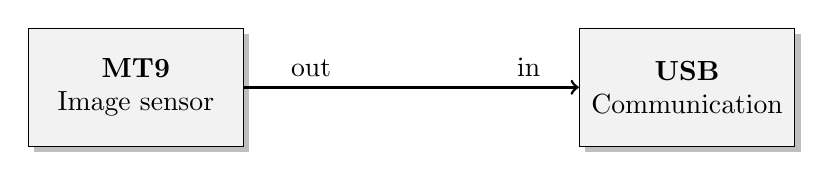
\begin{tikzpicture}[node distance=8cm]

\tikzset{blocstyle/.style={block,rectangle,minimum height=1.5cm,text width=2.5cm}};

% blocks
\node[blocstyle] (bloc1) {\textbf{MT9}\\Image sensor};
\node[blocstyle] (bloc2) at (7,0) {\textbf{USB}\\Communication};

% Flow to
\path[connect,->] (bloc1.east) -- node[above,pos=0.2]{out} node[above,pos=0.85]{in} (bloc2.west);

\end{tikzpicture}
\caption{Details on flow connexion}
\end{figure}

\subsection{Create the project and configure platform}

\textbf{setenv}\\

Firstly, you need to create the project in an empty directory :

\begin{sample}
> mkdir tuto1\\
> cd tuto1\\
> \textbf{gpnode newproject} -n tuto1
\end{sample}

After that, you should have a file named \emph{tuto1.node} in the current directory. This file is the project file and contain the definition of the node. A node in GPStudio is a physical node, it can be a smart camera or a sensor. You can have only one project file per directory and gpnode always works on the project in the current directory. The directory name can be different that the project name, but you should not modify the name of the project file.\\

The next thing to do is to specify the platform that you want to use for this project. You can do it with :

\begin{sample}
> \textbf{gpnode setboard} -n dreamcam\_c3
\end{sample}

`dreamcam\_c3' corresponds to a DreamCam platform with Cyclone III FPGA. The board support package for the `dreamcam\_c3' camera is located at :

\emph{<gps-root>/support/board/dreamcam\_c3/dreamcam\_c3.dev}

DreamCam is now set as a target platform. You can check that with the command command{showboard} :

\begin{sample}
> \textbf{gpnode showboard}
\begin{Verbatim}
dreamcam_c3
\end{Verbatim}
\end{sample}

To have the complete list of supported board, use the gplib tool with the command \textbf{listboard} :

\begin{sample}
> \textbf{gplib} \textbf{listboard}
\begin{Verbatim}
arrow_sockit de0nano dreamcam_c3 stratixcam_s4
\end{Verbatim}
\end{sample}

\subsection{Add IO support that you need}
Until now, we only specify the Dreamcam as platform, but it is a modular one, you can use different types of image sensor and communication. We need to define witch one we want to use by adding the support of theses peripherals. \\

You can use this command to know the available ios for the platform that you have specified before :
\begin{sample}
> \textbf{gpnode listavailableio}
\begin{Verbatim}
led mt9 e2v ethernet usb
\end{Verbatim}
\end{sample}

For image sensor, you have two possibilities, mt9 from Aptina or e2v. For this example, we choose mt9 :

\begin{sample}
> \textbf{gpnode addio} -n mt9
\end{sample}

By adding mt9 IO, gpnode fetches the name of the driver to use with this IO and copies the hardware driver files implementation. Like that, it allows you to use this image sensor in order to acquire pictures.\\

Now, to enable a communication, you have the choice between Ethernet or USB. Choose USB support :

\begin{sample}
> \textbf{gpnode addio} -n usb
\end{sample}

You can view the list of ios supports with the command \textbf{showio} :

\begin{sample}
> \textbf{gpnode showio}
\begin{Verbatim}
ios :
  + mt9 [mt9]
  + usb [usb_cypress_CY7C68014A]
\end{Verbatim}
\end{sample}

\subsection{Connect block flow}
To obtain a simple image sent from the image sensor to USB communication, we need a direct connection between `mt9' output image flow and `usb' input flow. To see flows that could be connected of a block, use the command \textbf{showblock} with a filter for looking only flows :

\begin{sample}
> \textbf{gpnode showblock} -n mt9 -f flows
\begin{Verbatim}
flows :
    -------------       
    |    mt9    |  out  
    |           |------>
    -------------
\end{Verbatim}
\end{sample}

And for usb block :

\begin{sample}
> \textbf{gpnode showblock} -n usb -f flows
\begin{Verbatim}
flows :
       -------------        
  in0  |           |  out0  
------>|           |------->
  in1  |           |  out1  
------>|           |------->
  in2  |    usb    |        
------>|           |        
  in3  |           |        
------>|           |        
       -------------
\end{Verbatim}
\end{sample}

So we want to have this graph of connection :
\begin{figure}[h!]
\centering
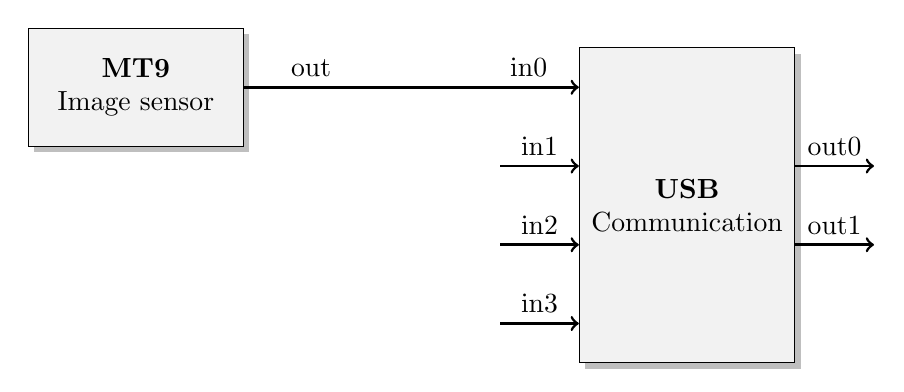
\begin{tikzpicture}[node distance=8cm]

\tikzset{blocstyle/.style={block,rectangle,minimum height=1.5cm,text width=2.5cm}};

% blocks
\node[blocstyle] (bloc1) {\textbf{MT9}\\Image sensor};
\node[blocstyle,minimum height=4cm] (bloc2) at (7,-1.5) {\textbf{USB}\\Communication};

% Flow to
\path[connect,->] (bloc1.east) -- node[above,pos=0.2]{out} node[above,pos=0.85]{in0} ([yshift=1.5cm]bloc2.west);
\path[connect,<-] ([yshift=0.5cm]bloc2.west) -- node[above]{in1} ++(-1,0);
\path[connect,<-] ([yshift=-0.5cm]bloc2.west) -- node[above]{in2} ++(-1,0);
\path[connect,<-] ([yshift=-1.5cm]bloc2.west) -- node[above]{in3} ++(-1,0);

\path[connect,->] ([yshift=0.5cm]bloc2.east) -- node[above]{out0} ++(1,0);
\path[connect,->] ([yshift=-0.5cm]bloc2.east) -- node[above]{out1} ++(1,0);

\end{tikzpicture}
\caption{Details on flow connexion}
\end{figure}

To do it, you need to add a connection with the command \textbf{connect} :
\begin{sample}
> \textbf{gpnode connect} -f mt9.out -t usb.in0
\end{sample}

To check the effective connection, it is possible to print the list of connection with \textbf{showconnects} :
\begin{sample}
> \textbf{gpnode showconnects}
\begin{Verbatim}
connects :
  + mt9.out -> usb.in0 (msb)
\end{Verbatim}
\end{sample}

Your project is now fully configured. The next step is to generate code dedicated to the platform. We do it in a `build' subdirectory :

\begin{sample}
> \textbf{gpnode generate} -o build
\end{sample}

After that, a subdirectory `build' is created in your project directory with the following files :

\begin{figure}[h]
\dirtree{%
.1 tuto1/.
   .2 tuto1.node\DTcomment{project file}.
   .2 \bfseries build/\DTcomment{output directory}.
        .3 top.vhd\DTcomment{generated top level}.
        .3 ci.vhd\DTcomment{generated CI block}.
        .3 pi.vhd\DTcomment{generated PI block}.
        .3 fi.vhd\DTcomment{generated FI block}.
        .3 node\_generated.xml\DTcomment{definition of the internal node}.
        .3 Makefile\DTcomment{Makefile}.
        .3 Makefile.local\DTcomment{paths for Makefile}.
        .3 params.h\DTcomment{addresses of each internal registers}.
        .3 \bfseries IP/ \DTcomment{local copy of used IPs}.
           .4 IP1.
           .4 IP2.
           .4 IP....
}
\caption{Files tree of the main distribution of GPStudio}
\label{fig:archivetree}
\end{figure}

The produced Makefile offers you several commands :
\begin{itemize}
\item \textbf{generate} : regenerate the project if you made some modification
\item \textbf{compile} : launch the compiler for your platform and produce a bitstream for the FPGA
\item \textbf{send} : configure the connected camera with the bitstream
\item \textbf{view} : launch the viewer
\end{itemize}

To launch the compilation process, go into the build directory, and start the command `compile' :

\begin{sample}
> cd build/\\
> make compile
\end{sample}

After few minutes, your project is now compile and ready to send to the camera.

First of all, powered up the DreamCam. Then, connect an USB cable from your computer to the USB communication board at the rear of the camera. Connect a second one to the internal JTAG near the power board.

To configure the FPGA with the generated bitstream, use the `send' rule of the Makefile :

\begin{sample}
> make send
\end{sample}

This command needs only few seconds to be done. If no errors appear, camera is ready and you can launch the debugger viewer to test your project, \textbf{gpviewer}.

\begin{sample}
> make view
\end{sample}

\section{Adding a process from GPStudio library}
In this second part, we want to add some processing between the image sensor and the communication to obtain a smart camera and not only a `webcam'.

\begin{figure}[h!]
\centering
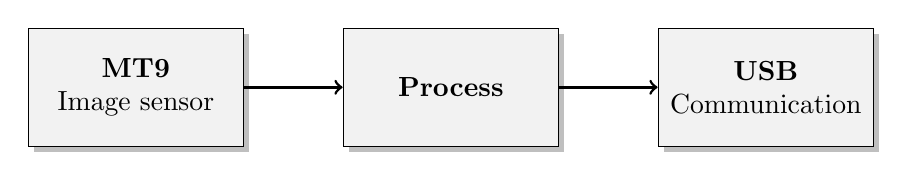
\begin{tikzpicture}[node distance=8cm]

\tikzset{blocstyle/.style={block,rectangle,minimum height=1.5cm,text width=2.5cm}};

% blocks
\node[blocstyle] (bloc1) {\textbf{MT9}\\Image sensor};
\node[blocstyle] (blocproc) at (4,0) {\textbf{Process}};
\node[blocstyle] (bloc2) at (8,0) {\textbf{USB}\\Communication};

% Flow to
\path[connect,->] (bloc1) -- (blocproc);
\path[connect,->] (blocproc) -- (bloc2);

\end{tikzpicture}
\caption{Details on flow connexion}
\end{figure}

\subsection{Add process that you need}
Check process that could be use :

\begin{sample}
> \textbf{gplib listprocess}
\begin{Verbatim}
conv gradienthw histogramhw hog lbp normhw roi slidevm
\end{Verbatim}
\end{sample}

For example, we add a gradienthw as process block and we call it `process1' :

\begin{sample}
> \textbf{gpnode addprocess} -n process1 -d gradienthw
\end{sample}

To have the list of process in the project, just type :

\begin{sample}
> \textbf{gpnode showprocess}
\begin{Verbatim}
process :
  + process1 [gradienthw]
\end{Verbatim}
\end{sample}
  

\subsection{Connect process flow}

\begin{sample}
> \textbf{gpnode showblock} -n process1 -f flows
\begin{Verbatim}
flows :
           ------------------
  in (16)  |                |  magnitude (16)
---------->|                |----------------->
           |    process1    |    angle (16)
           |                |----------------->
           ------------------
\end{Verbatim}
\end{sample}

\begin{figure}[h!]
\centering
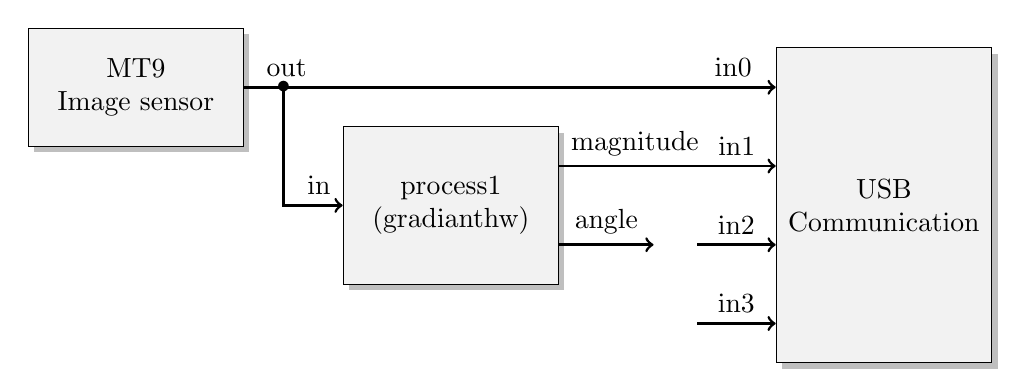
\begin{tikzpicture}[node distance=8cm]

\tikzset{blocstyle/.style={block,rectangle,minimum height=1.5cm,text width=2.5cm}};

% blocks
\node[blocstyle] (bloc1) {MT9\\Image sensor};
\node[blocstyle,minimum height=4cm] (bloc2) at (9.5,-1.5) {USB\\Communication};
\node[blocstyle,minimum height=2cm] (process1) at (4,-1.5) {process1\\(gradianthw)};

% Flow to
\path[connect,->] (bloc1.east) -- node[above,pos=0.08]{out} node[above,pos=0.92]{in0} ([yshift=1.5cm]bloc2.west);
\path[connect,->] ([yshift=0.5cm]process1.east) -- node[above,pos=0.35]{magnitude} node[above,pos=0.82]{in1} ([yshift=0.5cm]bloc2.west);
\path[connect,->] ([yshift=-0.5cm]process1.east) -- node[above]{angle} ++(1.2,0);
\path[connect,<-] ([yshift=-0.5cm]bloc2.west) -- node[above]{in2} ++(-1,0);
\path[connect,<-] ([yshift=-1.5cm]bloc2.west) -- node[above]{in3} ++(-1,0);

\path[connect,->] (bloc1.east) -- ++(0.5,0) node{$\bullet$} |- node[above,pos=0.8]{in} (process1);

\end{tikzpicture}
\caption{Details on flow connexion}
\end{figure}


\begin{sample}
> \textbf{gpnode connect} -f mt9.out -t process1.in\\
> \textbf{gpnode connect} -f process1.magnitude -t usb.in1
\end{sample}

\begin{sample}
> \textbf{gpnode showconnects}
\begin{Verbatim}
connects :
  + mt9.out -> usb.in0 (msb)
  + mt9.out -> process1.in (msb)
  + process1.magnitude -> usb.in1 (msb)
\end{Verbatim}
\end{sample}

\section{Creating custom process}
\subsection{Simple process}
A tool is done for custom block process, \textbf{gpproc}. It allows to describe interfaces of your process and provide a template to fill with your code.

In your node directory, create a new directory with the process name and add a process project :
\begin{sample}
> mkdir myprocess \\
> cd myprocess \\
> \textbf{gpproc new} -n myprocess
\end{sample}

Creates flow interfaces :
\begin{sample}
> \textbf{gpproc addflow} -n in -d in -s 8 \\
> \textbf{gpproc addflow} -n out -d out -s 8
\end{sample}

Generates template in the directory hdl :
\begin{sample}
> \textbf{gpproc generate} -o hdl
\end{sample}

Adds generated files to the project :
\begin{sample}
> \textbf{gpproc addfile} -p hdl/myprocess.vhd -t vhdl -g hdl \\
> \textbf{gpproc addfile} -p hdl/myprocess\_process.vhd -t vhdl -g hdl
\end{sample}

Comes back to the node project and add your process :
\begin{sample}
> cd .. \\
> \textbf{gpnode addprocess} -n myprocess1 -d myprocess/myprocess.proc
\end{sample}

Connects it :
\begin{sample}
> \textbf{gpnode connect} -f mt9.out -t myprocess1.in \\
> \textbf{gpnode connect} -f myprocess1.out -t usb.in3
\end{sample}

Tests it :
\begin{sample}
> cd build \\
> make generate compile send view
\end{sample}


\subsection{Process with dynamic parameters}

Returns in the process definition directory and creates a parameter :
\begin{sample}
> cd myprocess \\
> \textbf{gpproc addparam} -n threshold\_reg
\end{sample}

A parameter is set by default as dynamic register, you just need to set a relative address :
\begin{sample}
> \textbf{gpproc setparam} -n threshold\_reg -r 0 \\
Warning (1) : Your relative adress is greater than the range of relative address (0 bits). \\
Please specify a new PI size address with : \\
gpproc setpisizeaddr -v 2
\end{sample}

Sets the size of PI address bus to 2 bits :
\begin{sample}
> \textbf{gpproc setpisizeaddr} -v 2
\end{sample}

Adds a property and link the register to this property :
\begin{sample}
> \textbf{gpproc addproperty} -n threshold -t int \\
> \textbf{gpproc setpropertymap} -n threshold\_reg -v threshold.value
\end{sample}

Generates template in the directory hdl and add the slave block :
\begin{sample}
> \textbf{gpproc generate} -o hdl \\
> \textbf{gpproc addfile} -p hdl/myprocess\_slave.vhd -t vhdl -g hdl
\end{sample}

Tests it :
\begin{sample}
> cd ../build \\
> make generate compile send view
\end{sample}

\end{document}
